
%%%%%%%%%%%%%%%%%%%%%%%%%%%%%%%%%%%%%%%%%%%%%%%%%%%%%%%%%%%%%%
%\section{Basic Research Questions and Their Evaluations}
\label{sec:hypotheses}

To evaluate the framework's usability for non-expert users, %we formulated the following hypotheses:
%\begin{enumerate}
%\item[\textbf{H1}] \textit{The user understands the symbolic planning concepts.} This allows us to verify, if the symbolic planning language (PDDL), to describe the world state in terms of object types, properties, generalised properties, and action models, in terms of preconditions and effects, can be adopted easily by non-expert users.
%\item[\textbf{H2}] \textit{The user is able to teach the robot an action model using the proposed framework.} This allows us to evaluate how users operate the framework.
%\end{enumerate} 
we conducted two qualitative user experiments to respond to the questions:
\begin{enumerate}
  \item[\textbf{Q1}] How do non-expert users adopt the automated planning language with its action model representation? (Section \ref{sec:Exp1})
  \item[\textbf{Q2}] Can users teach a robot action models for automated planning using the robot programming framework? (Section \ref{sec:Exp2})
\end{enumerate}
\begin{figure}[htp]
	\centering
	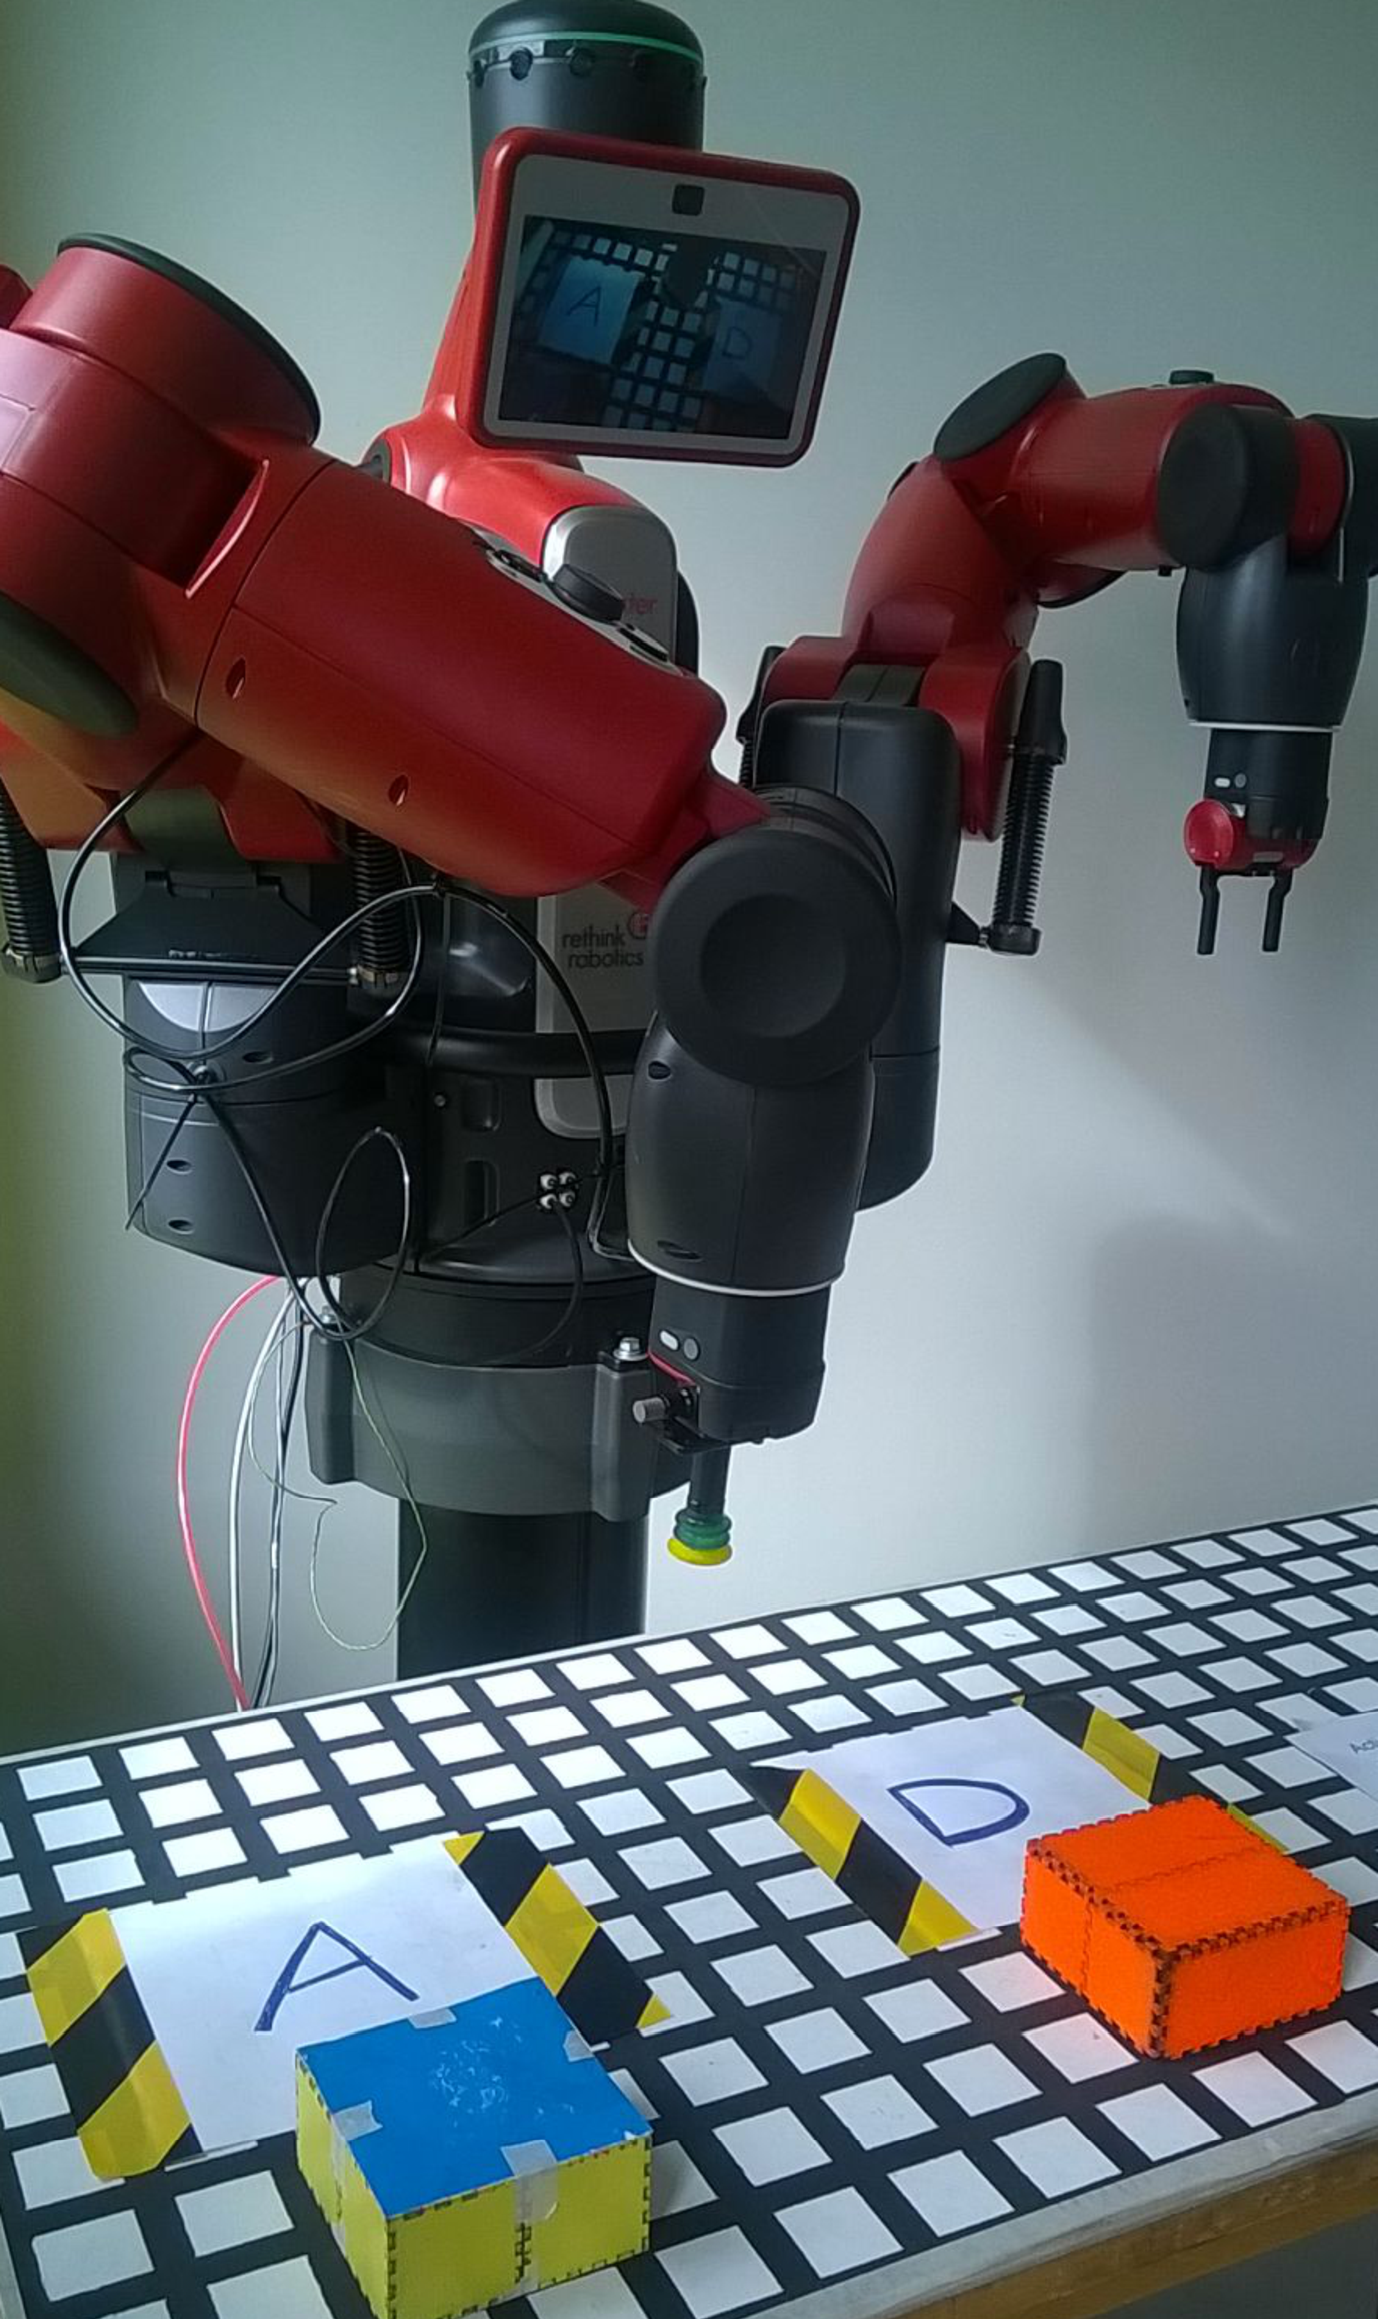
\includegraphics[width=.3\textwidth]{figures/experiment1}\hspace{1cm}%\hfill
	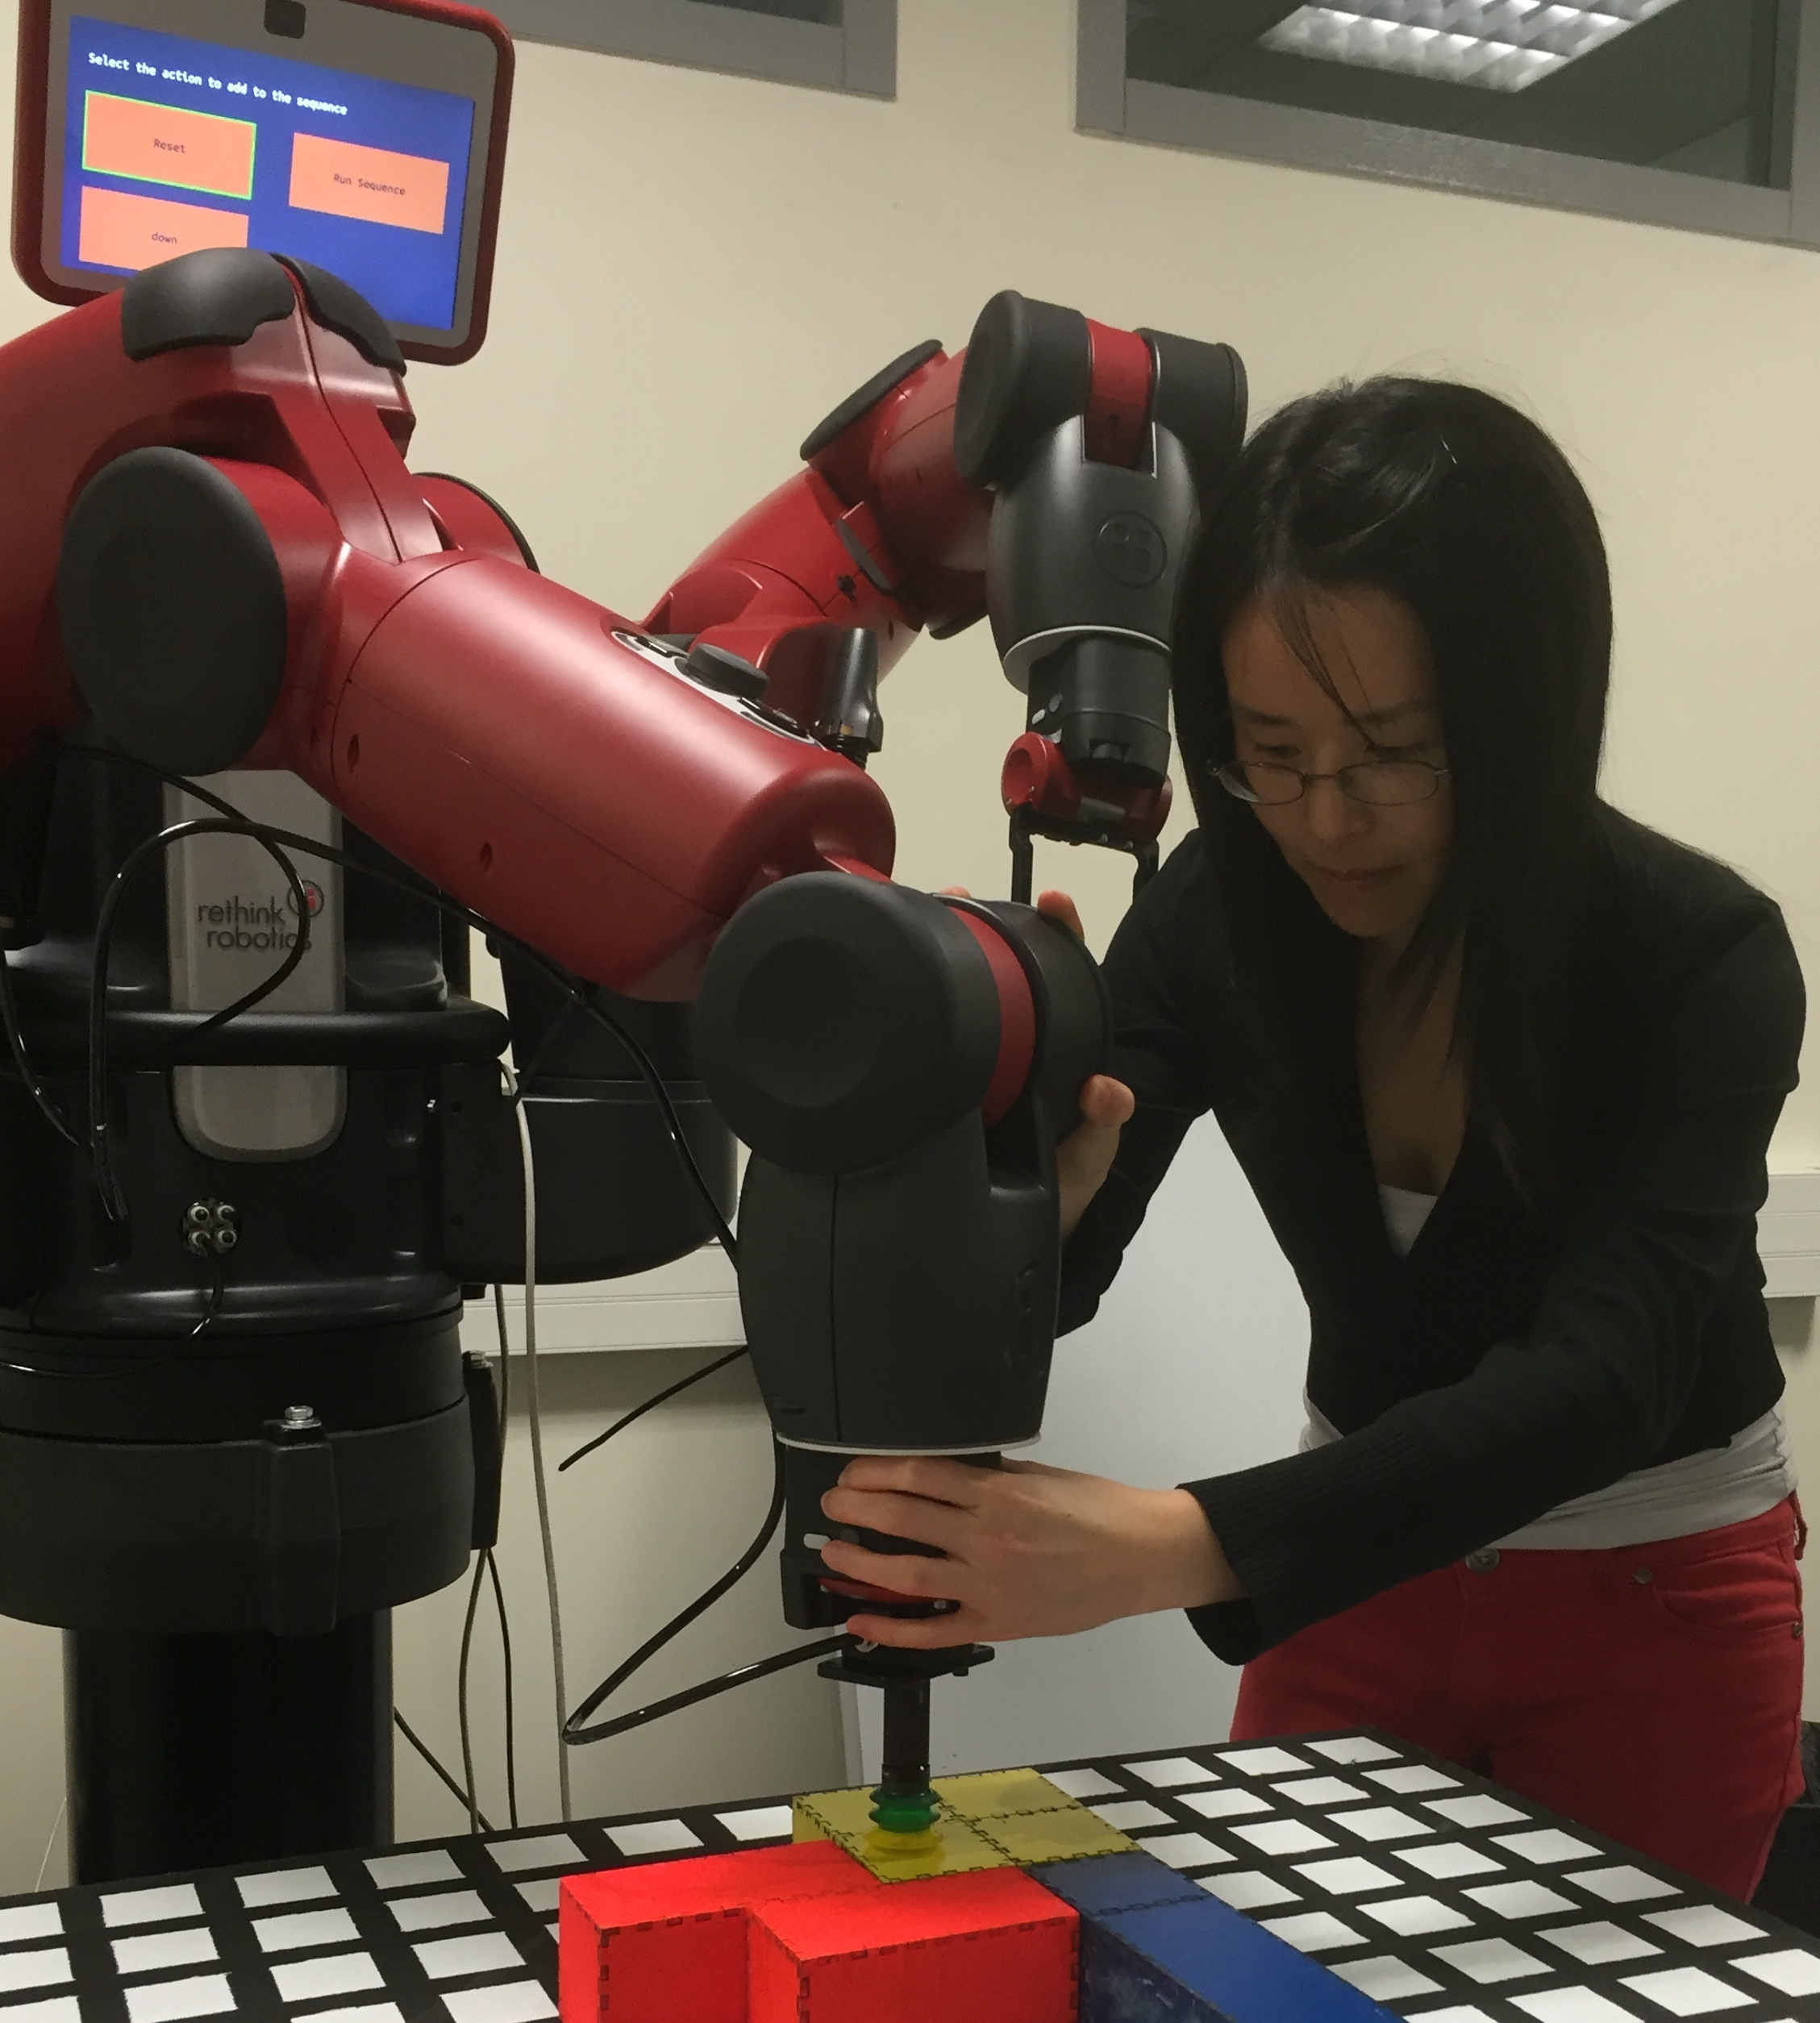
\includegraphics[width=.3\textwidth]{figures/experiment-setup2}
	
	\caption{Experimental setup for user studies on Programming by Demonstration of a move action by kinesthetic manipulation of the Baxter robot.}
	\label{fig:Baxter}
	
\end{figure}

The experimental context was designed around a Baxter robot (\fig{fig:Baxter}).
In both experiments, we included elements to assess the user's understanding of action models used by automated planners.
Understanding this symbolic representation is a key requirement to use the framework.
In the following sections, we briefly outline the experimental setup, measurements and results for each experiment.
 
% \begin{table}[t]
% \caption{Description of the world state in PDDL}
% \label{pddl_deschription}
% \begin{center}
% \begin{tabular}{l|l|l|l} \hline
%  \textbf{object name} & \textbf{type} & \textbf{property} & \textbf{generalised property} \\ \hline 
% redCube & cube & (at cube A) & (at ?cube ?posA)\\ \hline 
% A & position & (empty A) & (empty ?posA)\\ \hline 
% \end{tabular}\label{tab:pddl_deschription}
% \end{center}
% \end{table}

% Taken from Paper2 Basic research questions + experiments 1

\section{Experiment 1: Acceptance of Automated Planning and PDDL Concepts}\label{sec:Exp1}

% \section{How do non-expert users adopt the automated planning language with its action model representation?}
%%%%%%%% 1.25 pages %%%%%%%
In this experiment, we are addressing the following question:

\begin{enumerate}
	\item[\textbf{Q1}] How do non-expert users adopt the automated planning language with its action model representation?
\end{enumerate}

Users were introduced to a symbolic planning language (a simplified version of PDDL), involving the STRIPS formalism (\cite{fikes1971strips}) with type structures used in automated planning (\chapt{chap:Sota-AP}).
Users were instructed to describe world state configurations to the robot.
The goal was to assess the user's adoption of the planning concepts (object types, properties, generalised properties, action models) and to verify that the symbolic planning language is appropriate for non-expert users.

\begin{figure}[htp]
	\centering
	\begin{subfigure}[t]{0.24\textwidth}%
		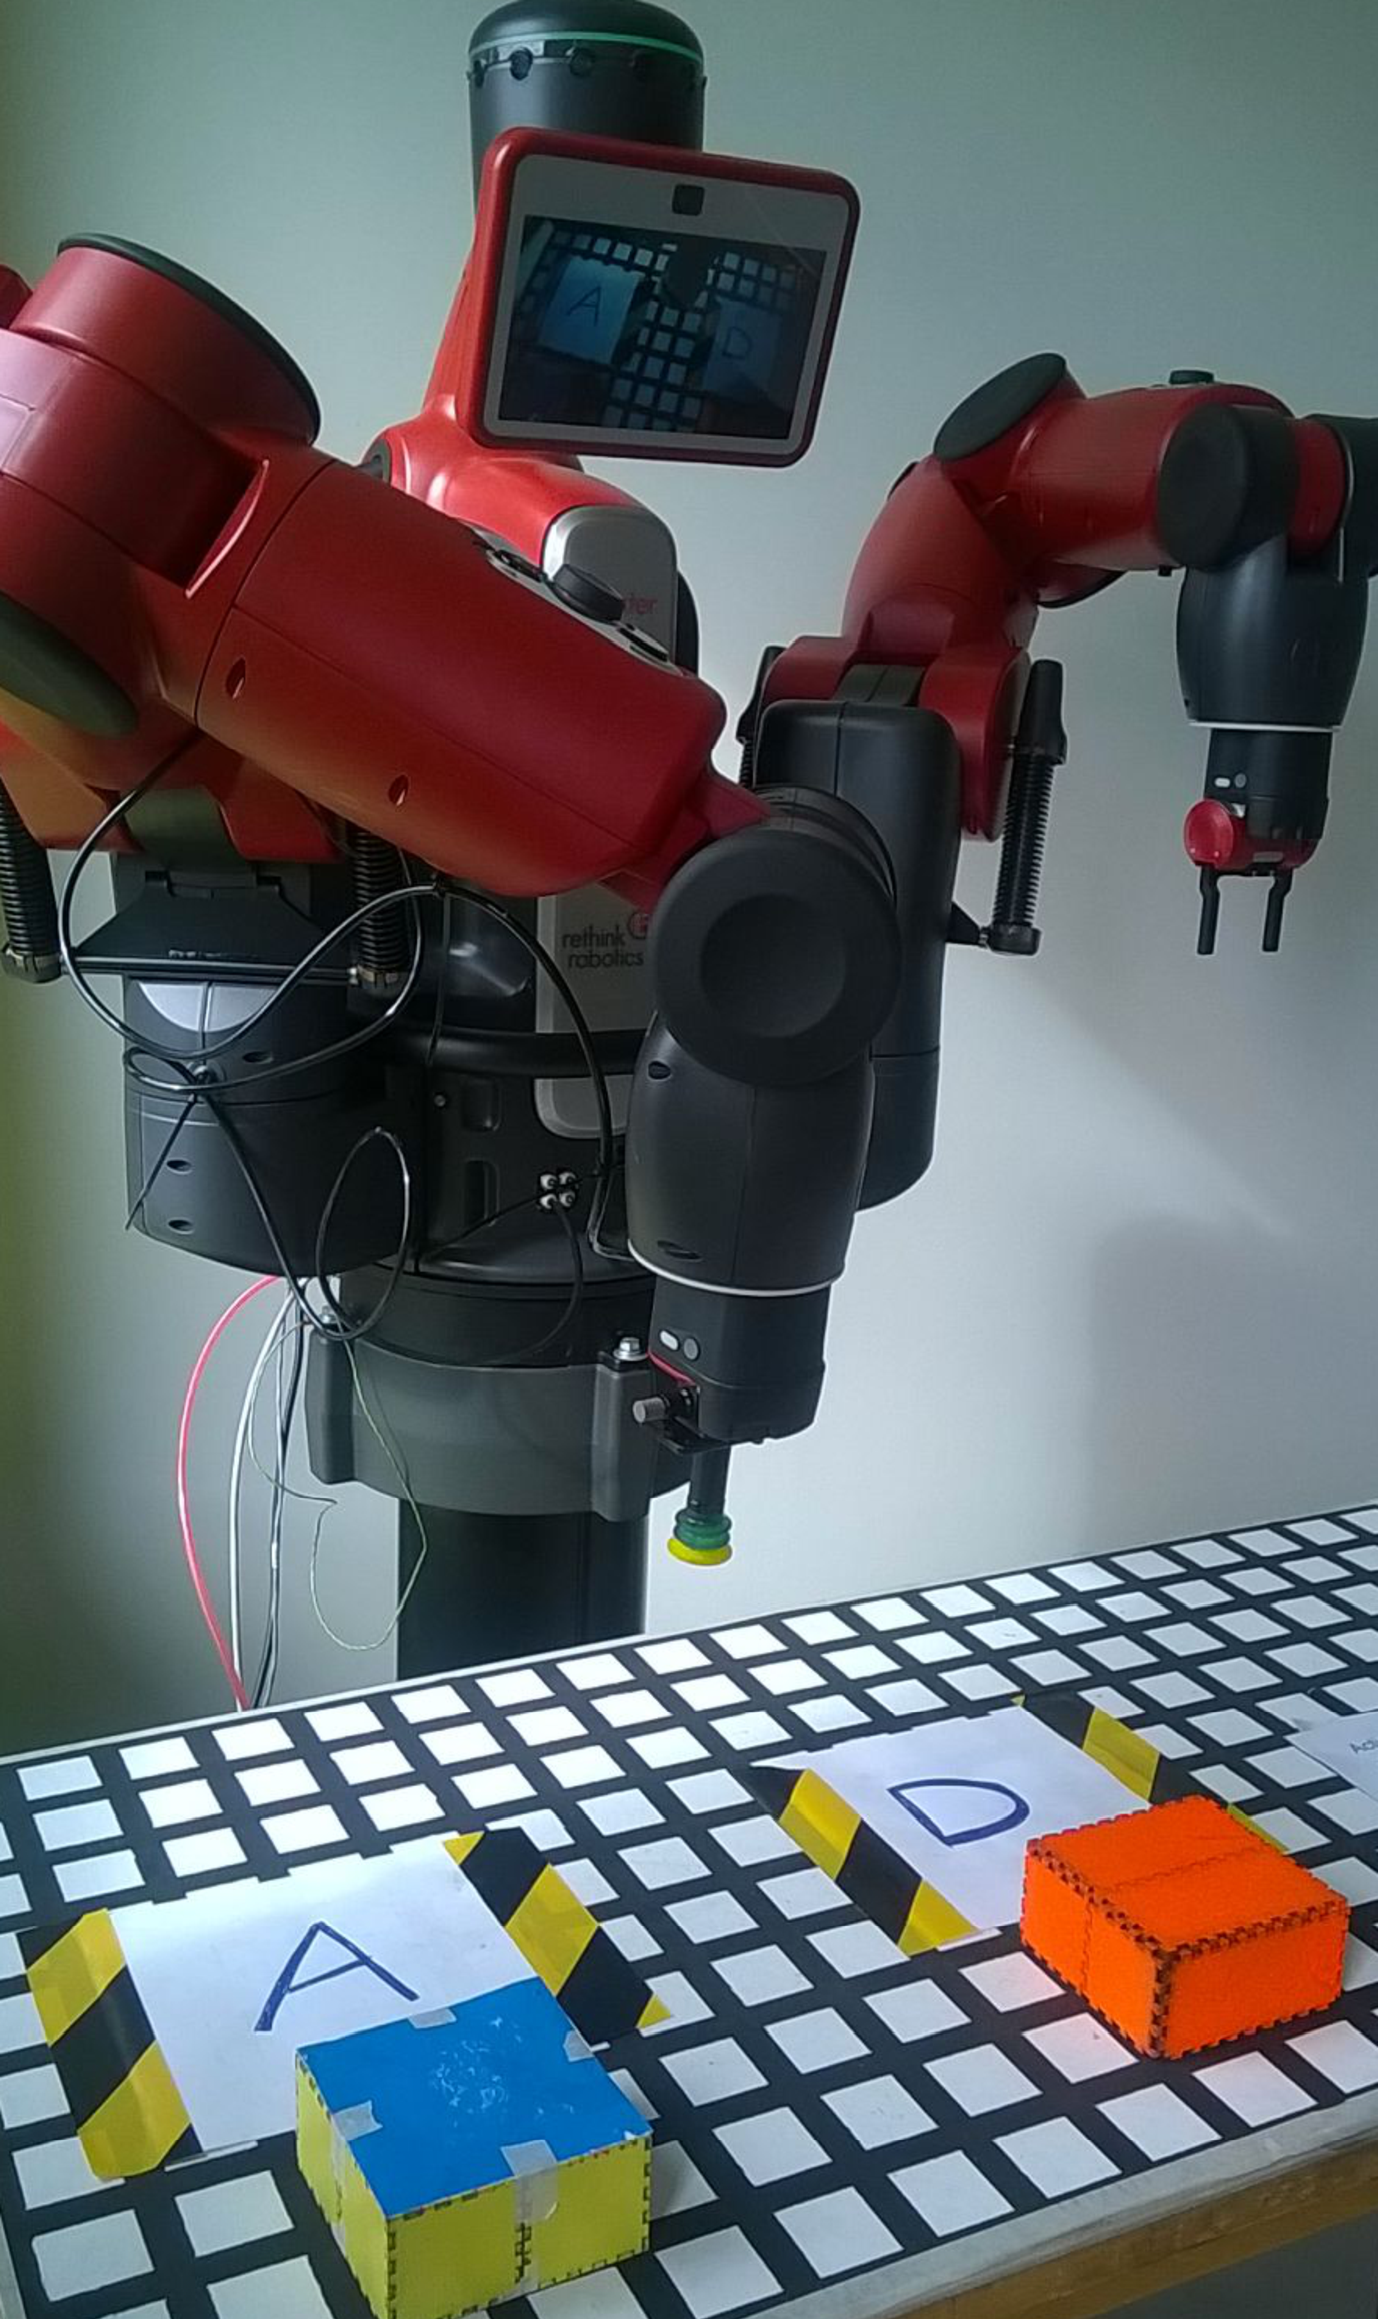
\includegraphics[width=\textwidth]{figures/experiment1}%
		\caption{Baxter robot}\label{fig:Baxter}%
	\end{subfigure}~~%
	\begin{subfigure}[t]{0.24\textwidth}%
		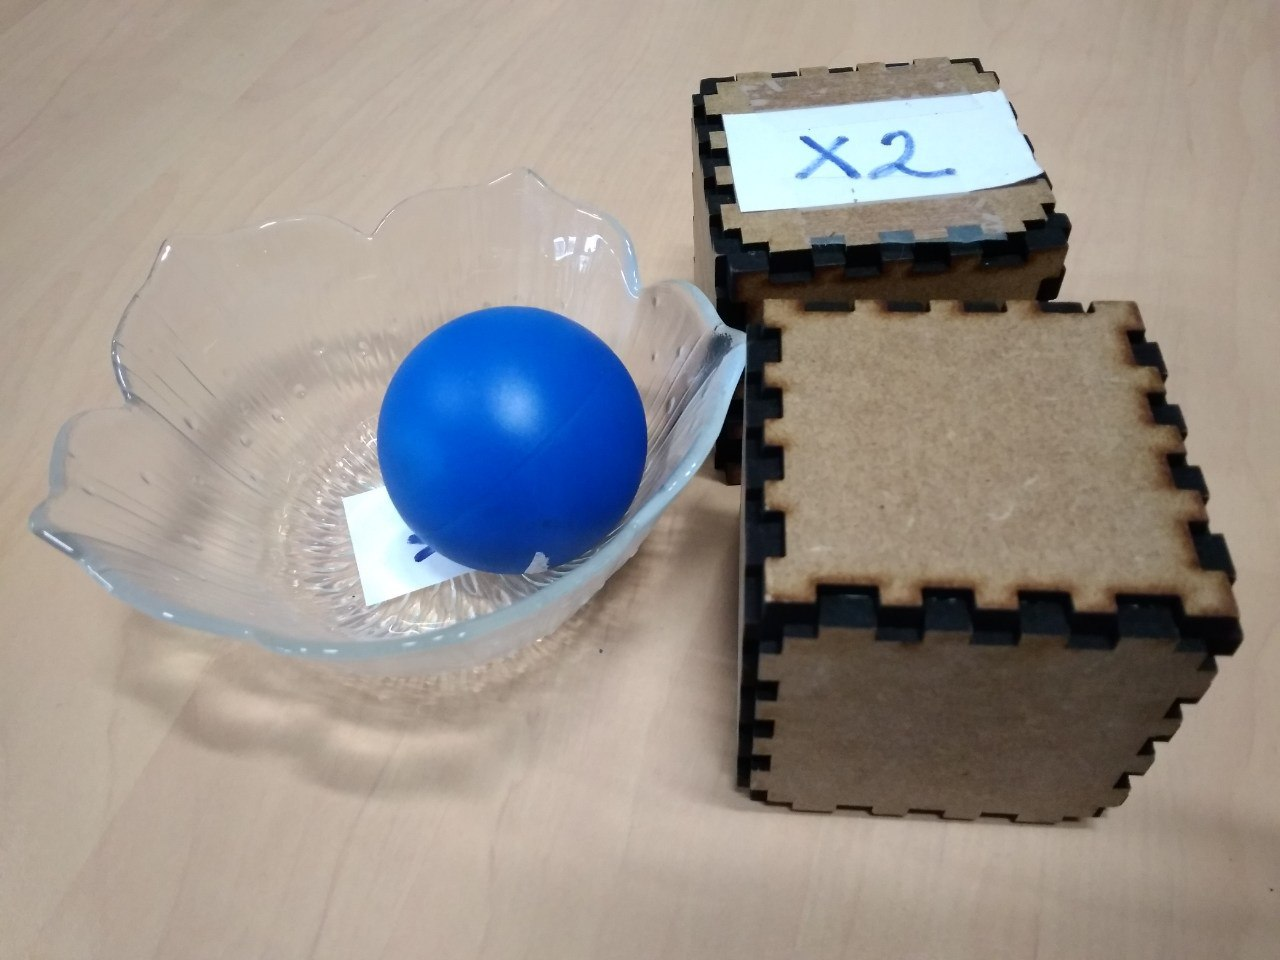
\includegraphics[width=\textwidth]{figures/exp1-setup}%
		\caption{Experiment 1 setup}\label{fig:exp1-setup}%  
	\end{subfigure} 	  
	\caption{Experimental setup for user studies.}
	\label{fig:pre-experiment}%
	% 	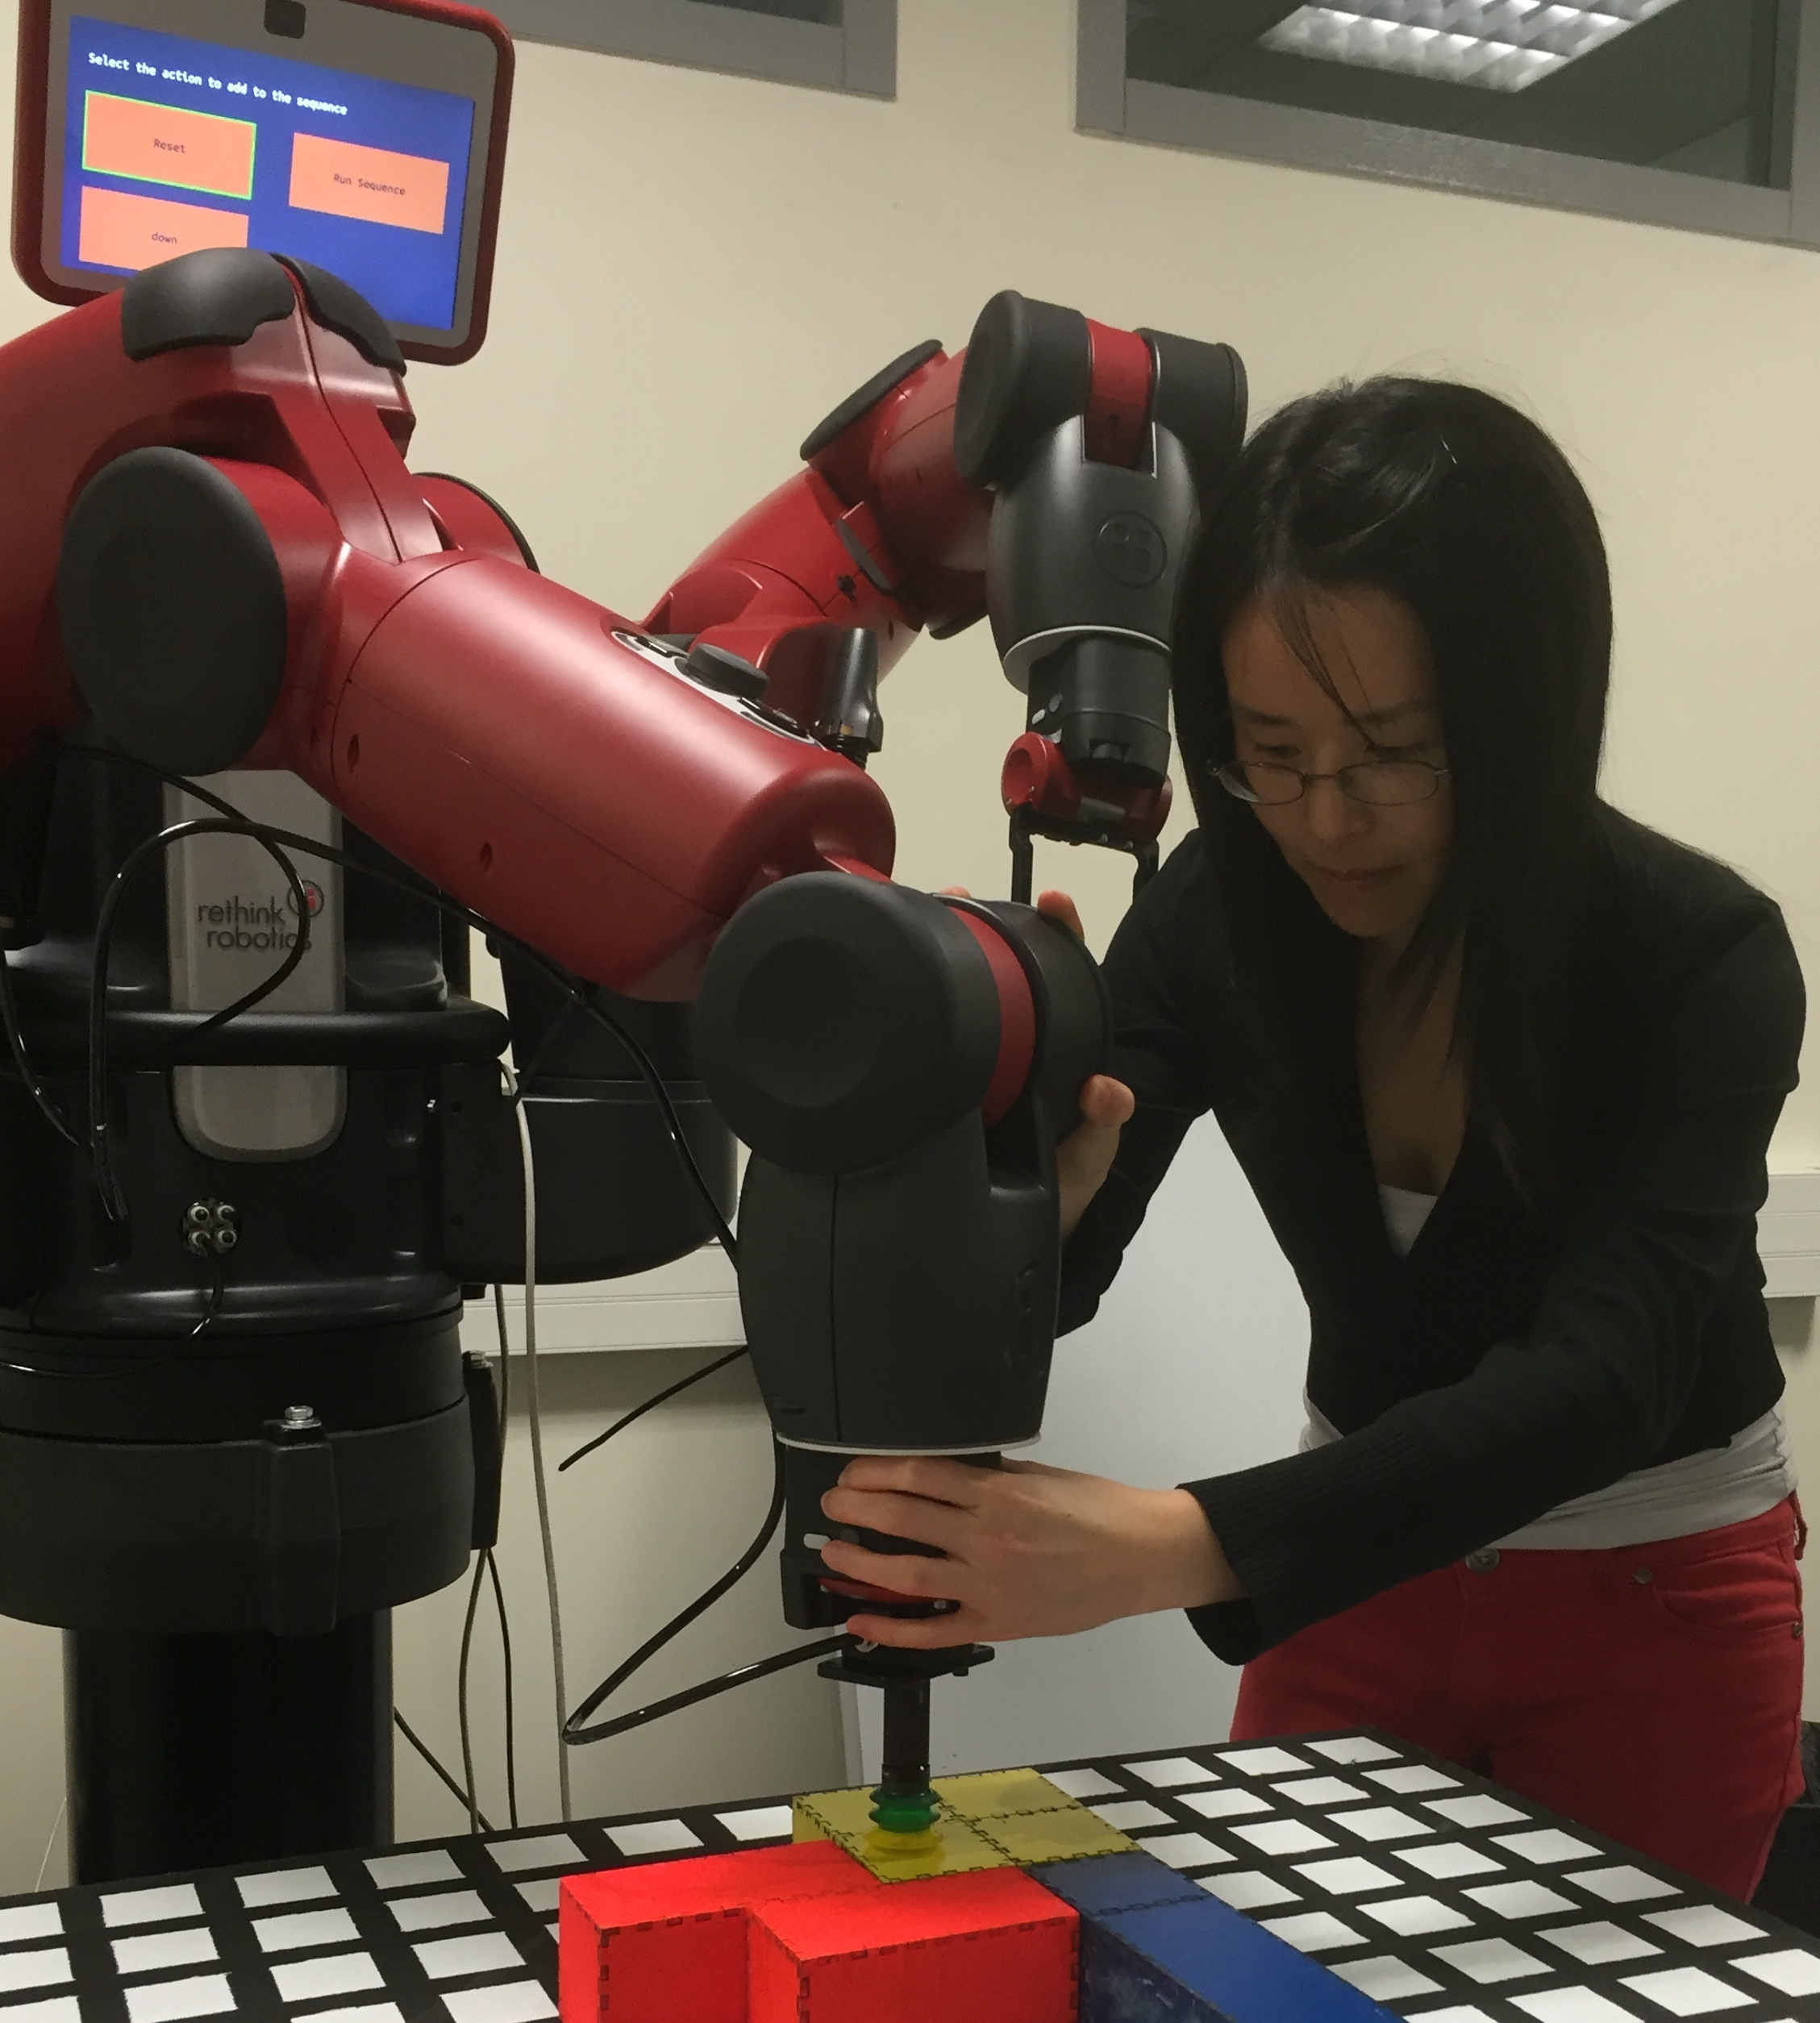
\includegraphics[width=.3\textwidth]{figures/experiment-setup2}
\end{figure}
\subsection{Experimental Setup \& Participants}
We recruited 10 participants (1 male, 9 female), who were sociology students at the Universit\'{e} Grenoble Alpes.
3 participants reported no programming experience, 6  had experience with office productivity software (`beginner'), and 1 had previously taken a programming course before (`advanced').

The experimental setup consisted of a 2x2 board (with positions A1, A2, B1, B2), 2 cubes, 1 ball, and 1 ball recipient in the form of a bowl (\fig{fig:exp1-setup}).
%The experimenter showed the participants a video of the Baxter robot \cite{Baxter}
The participants were given sheets with empty tables to complete for each task.
Each participant was allocated 1 hour, but the average duration of the experiment was 49 minutes.
At the end, participants were given a questionnaire related to their experience and their understanding of the learned planning language and concepts.
The participants' behaviour was observed by the experimenter and the experiment was recorded on camera.
The experimental protocol, questionnaire and additional material used can be found in Appendix \ref{app:exp1}.


%\begin{figure}[h]
%	\centering
%	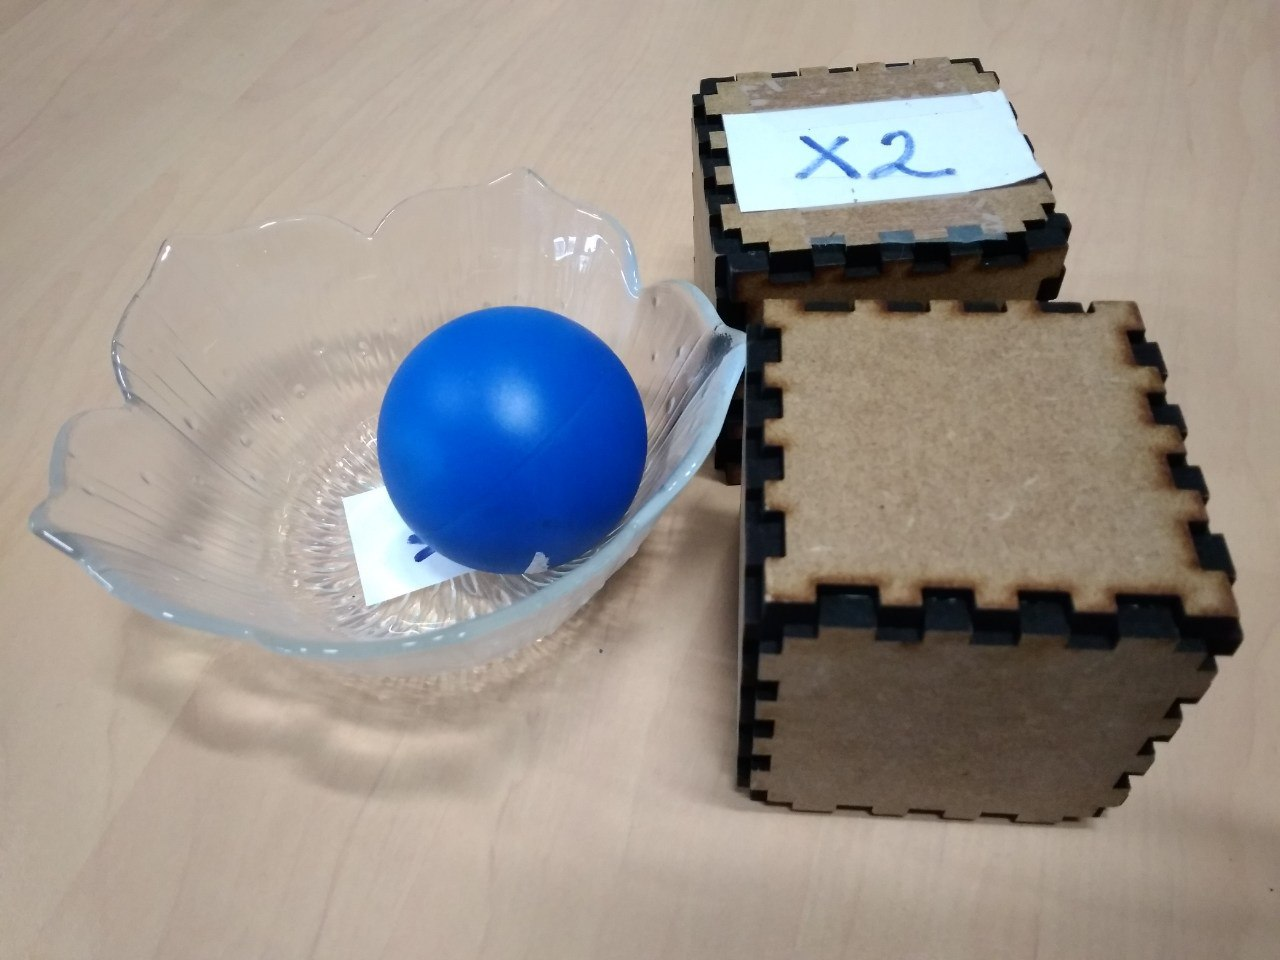
\includegraphics[width=0.65\linewidth]{figures/exp1-setup}
%	\caption{Experiment 1 setup consisted of a 2x2 board, 2 cubes, 1 ball, and 1 ball recipient}
%	\label{fig:exp1-setup}
%\end{figure}
 

\subsection{Experimental Design \& Measurements}
%After a short introduction to the Baxter robot, 
Users were told that they needed to use a symbolic planning language to describe the state of the world and the semantic meaning of actions to the robot. 
Throughout the experiment, users were faced with three different scenarios. 
\fig{fig:scenarios-exp1} shows an example of the experimental design, where the robot's action was to move the ball to an occupied position (B2). 
We evaluated their capability to apply the planning language to different situations.

\begin{figure}[h]
	\centering
	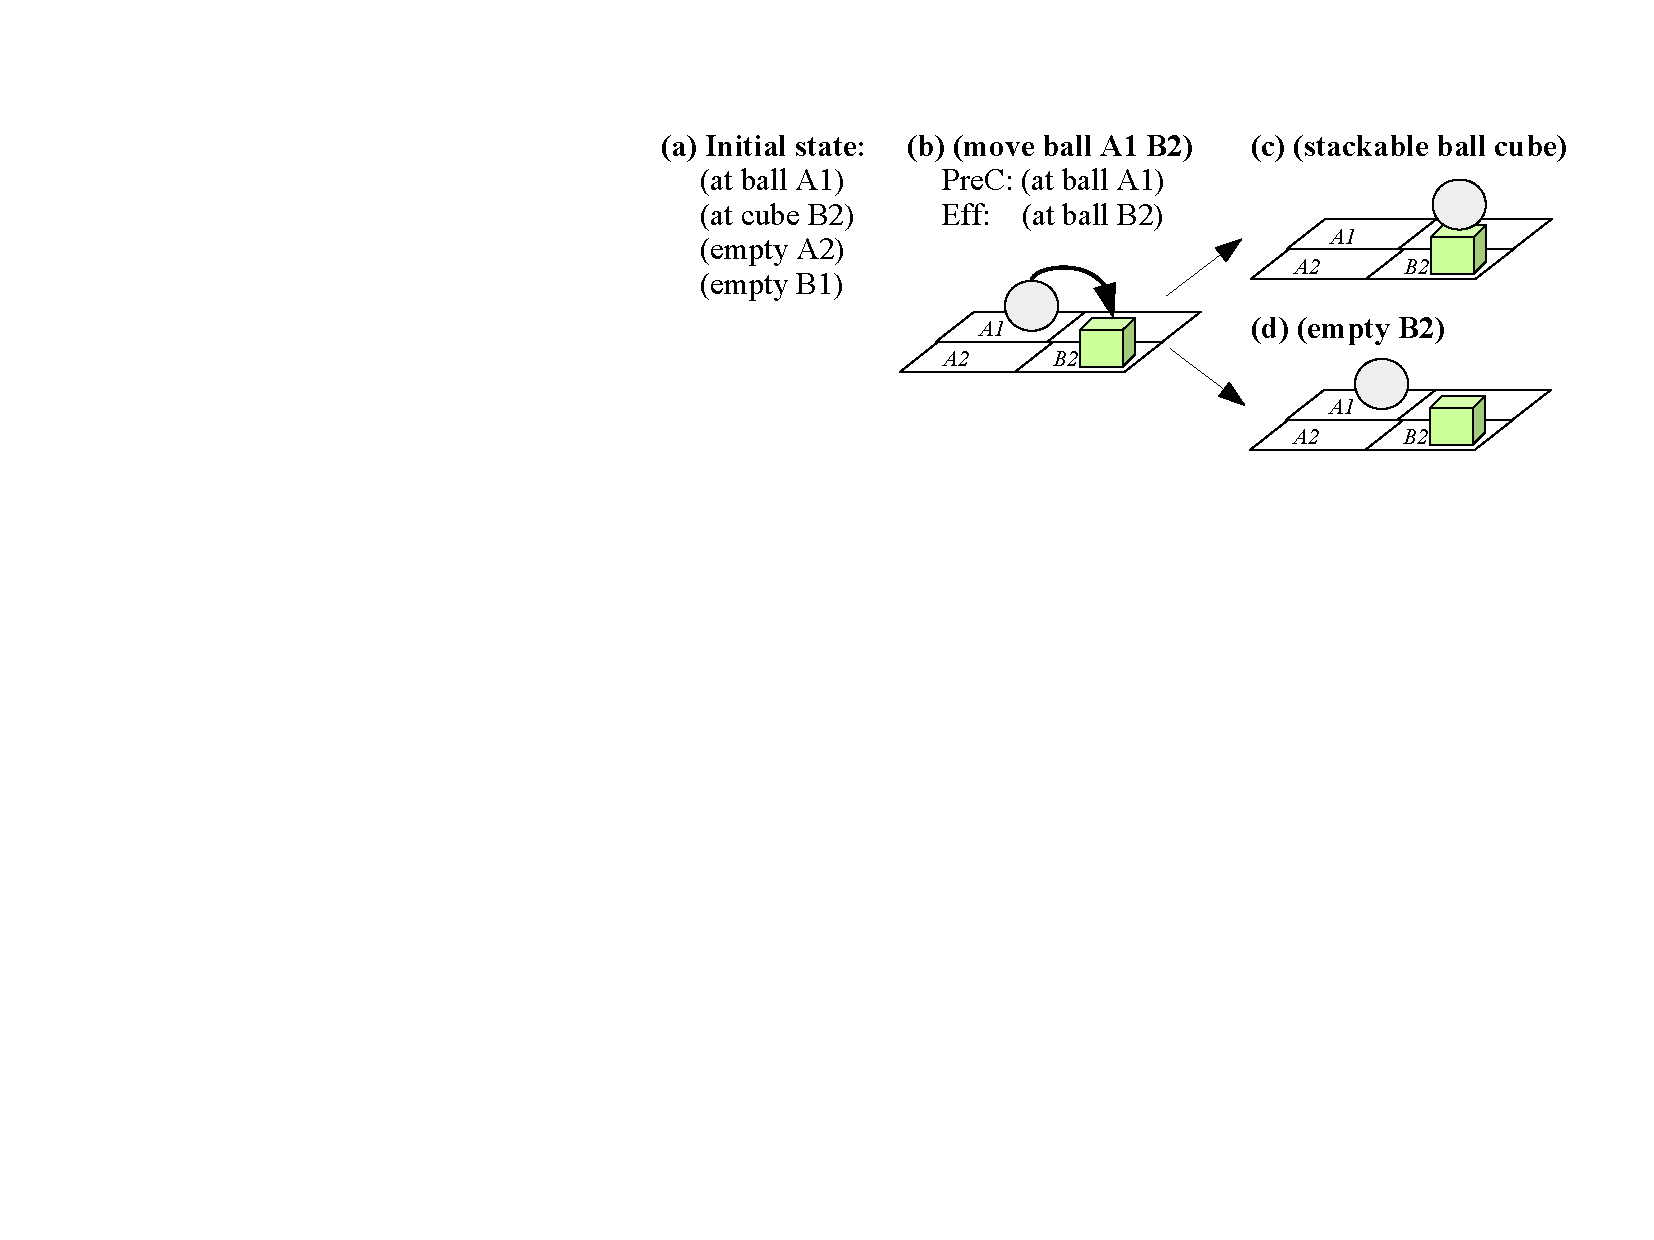
\includegraphics[width=0.75\linewidth]{figures/scenarios-exp1}
	\caption{Users were instructed to provide a description of (a) the initial state of the world and (b) an initial move action model.
		Then they derived additional preconditions for moving the ball from position A1 to B2: (c) \textit{(stackable ball cube)}: the ball can be stacked onto the cube, and (d) \textit{(empty B2)}: if the ball cannot be stacked, the target position should be empty.}
	\label{fig:scenarios-exp1}
\end{figure}

The experiment consisted of the following phases:
\begin{itemize}
%  \item{Introduction: After a short introduction to the Baxter robot \cite{Baxter}, users were told that they needed to use a planning language (STRIPS) to explain Baxter the state of the world and the semantic meaning of the actions.}
  \item{\begin{sloppypar} \textbf{Training:} Users were presented the symbolic planning language to describe object \textit{types} (\ie position, ball, cube, bowl) and predicates, which we called \textit{properties} (\ie \texttt{empty}, \texttt{at}, \texttt{stackable}, \texttt{is\_red}, \texttt{is\_blue}) to describe world states.
They were shown how to model a simple move action in terms of preconditions and effects (\fig{fig:action model}).
For all properties and actions, they had to use syntax of the form \texttt{name(arg1,arg2,\dots)} which users without a  Computer Science background might be unfamiliar with.
Additionally, they were introduced to the concepts of \textit{instantiated} and \textit{generalised} actions, which were equivalent to actions (\eg \texttt{move(X1)}) and planning operators (\eg \texttt{move(cube)}) respectively (\sect{subsec:Classical planning problem}).
In this phase, they were given a simple example of a cube at position A1 and moved to position B2.\end{sloppypar}
}
  \item{\textbf{Experimental test:} Users were presented a new world state that involved a cube, a bowl and a ball object. 
  	First they were instructed to provide a description of the initial state to the robot by using the symbolic planning language (\fig{fig:scenarios-exp1}a).
Then they were asked to define a move action model in terms of preconditions and effects (\fig{fig:scenarios-exp1}b).
In the following they were faced with 3 different scenarios to refine the preconditions of the move action.
Users derived a \texttt{(stackable ball cube)} property (\fig{fig:scenarios-exp1}c), which allowed a ball to be stacked on top of a cube.
When this property did not hold, users proposed the \texttt{empty} property (\fig{fig:scenarios-exp1}d), which the robot needed to verify before the action execution.
At each step, users had to give the generalised representation of the properties and action models.}
  \item{\textbf{Planning:} Users were presented a description of a new initial state of the world and a goal state.
They were asked to define an action sequence, that allows the transition from the initial to the goal state (similar to \fig{fig:planning-permutation}c), and explain their reasoning using the symbolic action model representation.
This optional test allowed us to further verify their understanding of the planning concepts, in particular action preconditions and effects.}
  \item{\textbf{Questionnaire:} At the end of the experiment users were given a questionnaire including 5 questions related to their experience, as well as 15 questions to evaluate their understanding of the learned planning language and concepts (\fig{fig:eEvaluation2}).
  For the latter, questions related to their understanding of the concepts presented at the start of the experiment (\eg `Explain the difference between the precondition and effect of an action'), syntax (\eg `Using the presented language, how do you describe the property \textit{cube X4 is on position B3}?'),
  %If move(CUBE) describes a move action, tick all statements that are true.
  logical reasoning 
  	(\eg `Is it possible to have \texttt{(empty A)} and \texttt{(at cube A)} in the same state?'), and other concepts (\eg `What is the generalised form of the given object property?').
  The complete questionnaire can be found in Appendix \ref{app:exp1}.}
   \item {\textbf{Debriefing:} Throughout the experiment, users were asked open-ended questions (\eg `What properties do you observe in the current world state?'), so that they were guided as little as possible and their responses were unbiased.
When the participant struggled to find an answer, the experimenter guided the participant in a possible direction (\eg `Why can the ball not be placed on the cube?').} 
\end{itemize}

\begin{figure}[ht]
	\centering
	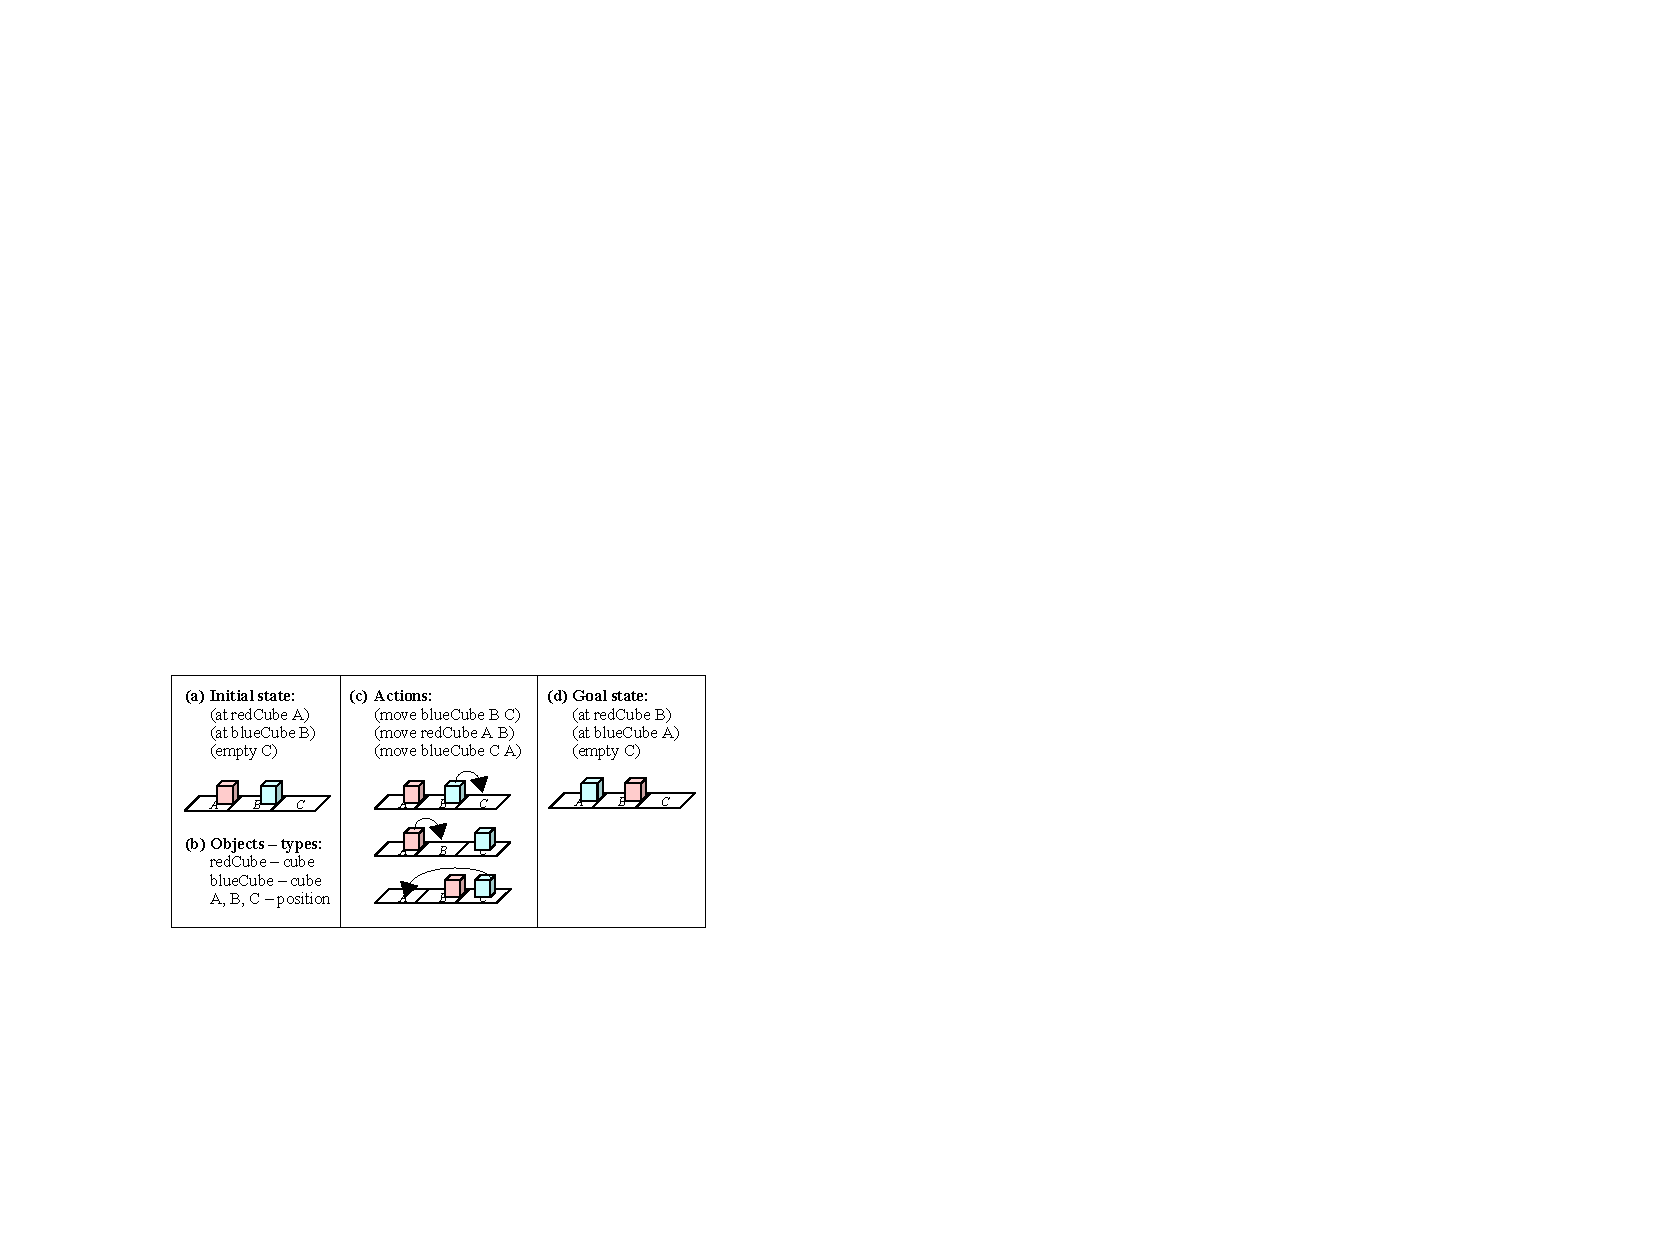
\includegraphics[width=0.7\linewidth]{figures/planning-permutation}
	\caption{Definition of a planning problem (a) properties describing the initial world state (b) object names and their types (c) instantiated actions (d) properties describing the goal state.}
	\label{fig:planning-permutation}
\end{figure}


\subsection{Results}
We did not observe any significant differences in the performance of users with or without programming experience.
9 (out of 10) participants found the symbolic representation of properties and actions easy to understand.
During the experimental test, the majority (9 or 90\%) of the participants managed to describe the complete world state using the correct syntax.
When faced with different scenarios to refine the move action model, 5 (or 50\%) of the participants struggled to formalise the \textit{stackable} condition in the symbolic language.
They provided alternative formulations related to the cube's properties (\eg `if the cube can hold the ball').
However, once the condition was defined, the majority (8 or 80\%) of the participants had little to no difficulties generalising properties, \eg defining planning operators (\fig{fig:action model}).
Due to time constraints, only 5 (or 50\%) participants were presented the planning phase.
All 5 encountered no problems when defining the action sequence to achieve the given goal.

In the questionnaire (\fig{fig:eEvaluation2}), the majority (9 or 90\%) of the participants understood the notion of states and object properties.
8 (or 80\%) correctly pointed out two properties that could not exist in the same state (\eg \texttt{(empty A)} and \texttt{(at cube A)}).
All participants gave correct explanations for preconditions and effects of action models, and provided correct examples.
9 (or 90\%) participants encountered difficulties during the experiment, 6 (or 60\%) stated problems with formalising the language, especially at the beginning of the experiment.
Half of the participants believed that they could apply this language on their own.
No participants believed that an `expert' programmer was required to learn the symbolic planning language, but 7 (or 70\%) participants believed that the minimum requirement was a `beginner' programming level, while 3 (or 30\%) believed that no programming experience was required at all.


\begin{figure}[ht]
	\centering
	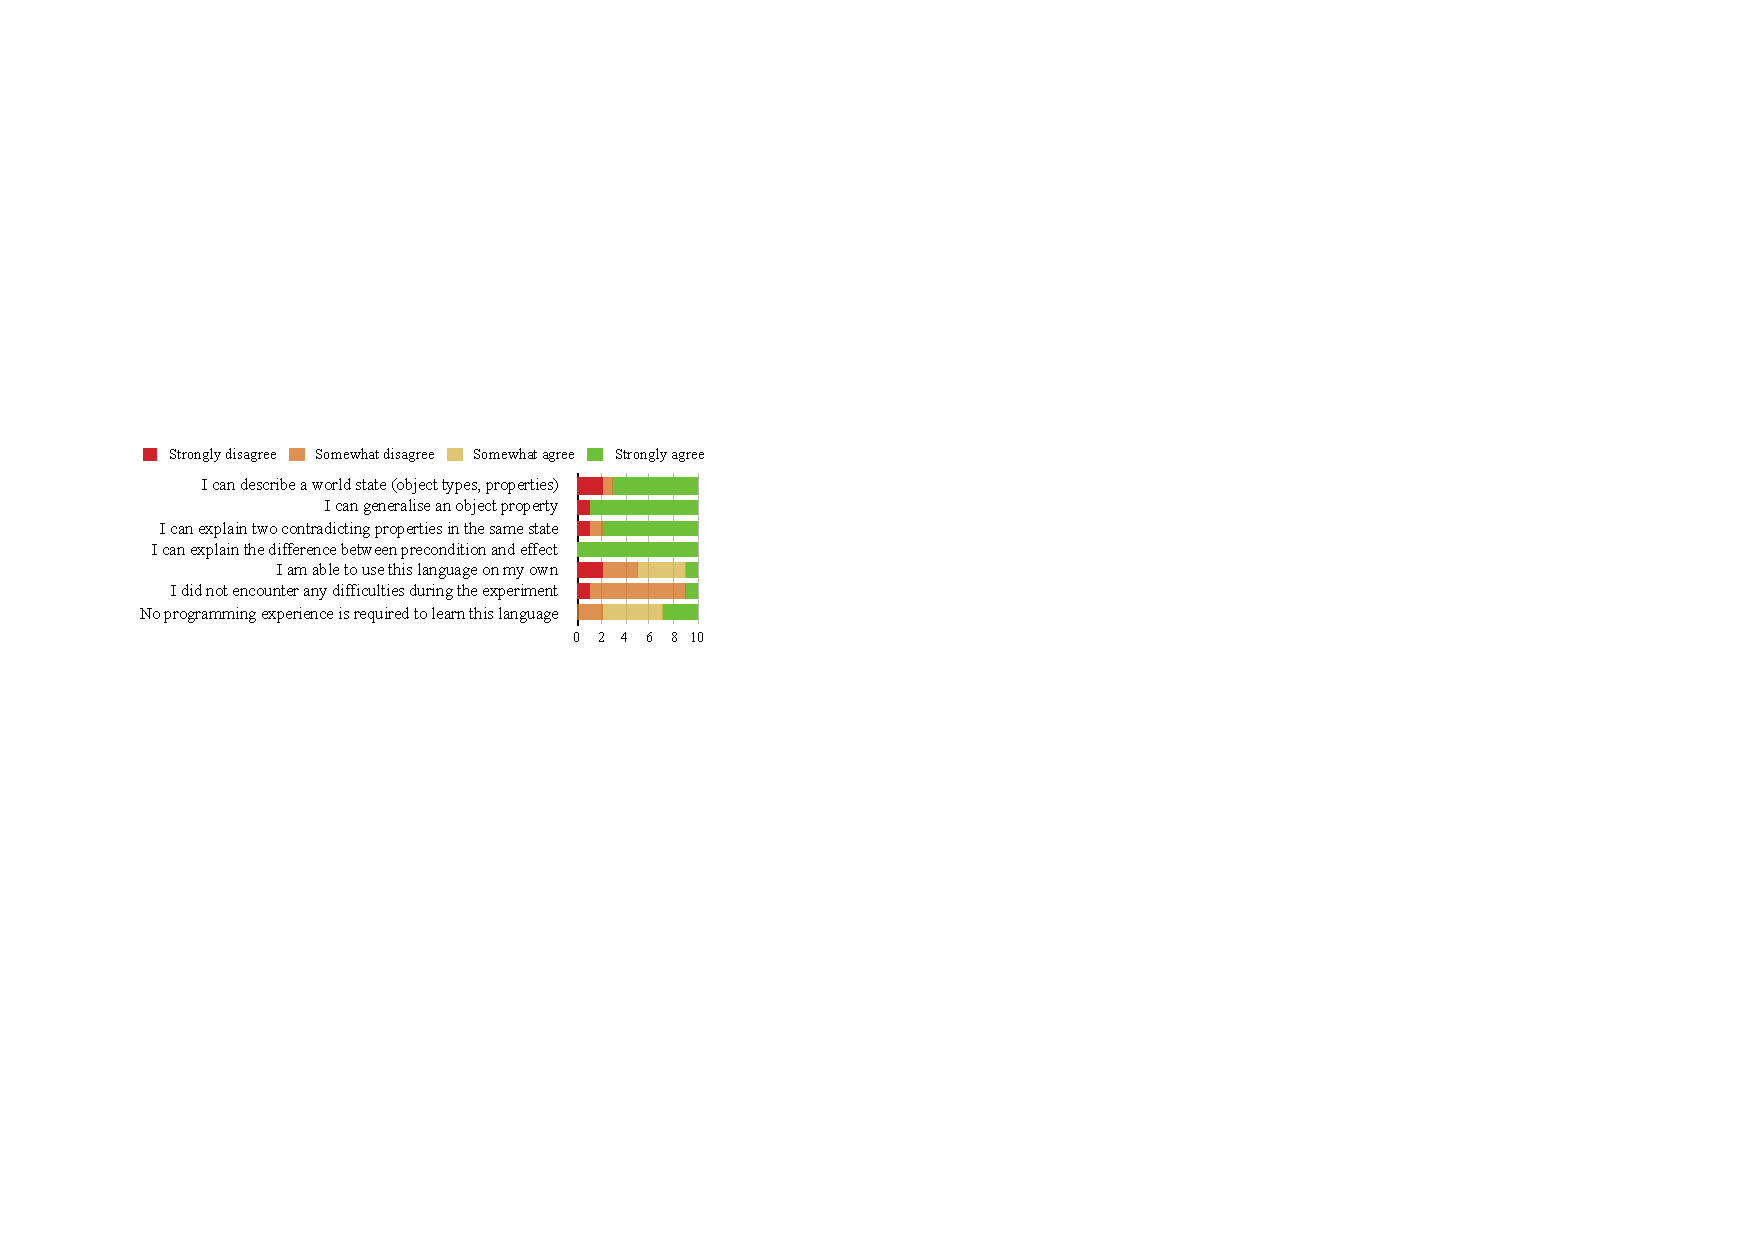
\includegraphics[width=0.85\linewidth]{figures/eEvaluation2}
	\caption{Summary of questionnaire responses: Extract of the 26 questions on the user's experience and understanding of the introduced planning language.}
	\label{fig:eEvaluation2}
\end{figure} 

\section{Experiment 2: Acceptance of the Robot Programming Framework}
\label{sec:Exp2}

In this experiment, we are addressing the following question:

\begin{enumerate}
  \item[\textbf{Q2}] Can users teach a robot action models for automated planning using the robot programming framework?
\end{enumerate}
\begin{sloppypar}
Users were presented a simulated implementation of the robot programming framework (\chapt{chap:Contribution}), and had to teach action models by kinesthetic manipulating a Baxter robot (\fig{fig:Baxter}). 
Users were instructed to demonstrate an atomic action and to assign preconditions and effects.
The goal was to assess the framework's usability and user's difficulties encountered when teaching action models.
At the end, participants were given a questionnaire related to their experience, their perceived understanding of the presented planning concepts and the usability of the framework.
The experimental protocol, questionnaire and additional material used can be found in Appendix \ref{app:exp2}.
In the following sections we briefly outline the experimental setup, measurements and results of the experiment.
%We then provide details on the partial implementation of the system used with the Wizard-of-Oz technique (\sect{ssec:WoZ}).
\end{sloppypar}

\subsection{Experimental Setup \& Participants}
We recruited 11 participants (7 male, 4 female), who were students and staff members at the Universit\'{e} Grenoble Alpes. 
6 participants reported programming experience with office productivity software (`beginner'), 2 had previously taken a programming course before (`advanced'), and 3 were pursuing studies in Computer Science (`expert').
%4 participants had previously heard of Automated Planning, but only 3 attended a related course.
The experiments were conducted using a Baxter robot (\fig{fig:Baxter}), mounted with a partial implementation of the framework.
The implemented functionalities included:
\begin{itemize}
	\item `learn new action': record the action demonstration
	\item `find a coloured object': apply the recorded action to an object of the specified colour
	\item `execute an action sequence': execute multiple actions
\end{itemize}

We used the Wizard-of-Oz technique to simulate the remaining functionalities (\eg `learn action preconditions and effects', `generate solution using a planner').
%Further details to the partial implementation are discussed in Section \ref{ssec:WoZ}.
Participants operated on a table with 2 positions D (for departure) and A (for arrival), 2 cubes (blue and red), that represented parts on an assembly line (\fig{fig:Baxter}). 
Each participant was allocated 1 hour, but the average duration was 29.5 minutes. 
The experiments were recorded, while the participant interacted with the robot. 


%The complete experimental protocol is shown in \fig{fig:Experimental protocol}. 
\subsection{Experimental Design \& Measurements}
The experiment scenario was set in a simulated assembly line, where objects of the same shape, but different colour arrived consecutively at the departure position D.
Users were told that objects were too heavy for human operators to move, hence needed to be handled by robots.
Also, due to the type of object, they should not be stacked.
Users had to teach Baxter the action for moving an object from D to arrival position A, for another maintenance task to be performed.
Throughout the experiment, users were faced with two different scenarios, where Baxter had to apply the learned move action. 
We evaluated the user's capability to refine action models and their associated conditions, when faced with different situations, and wanted to assess the framework's overall usability.

\begin{figure}[h]
	\centering
	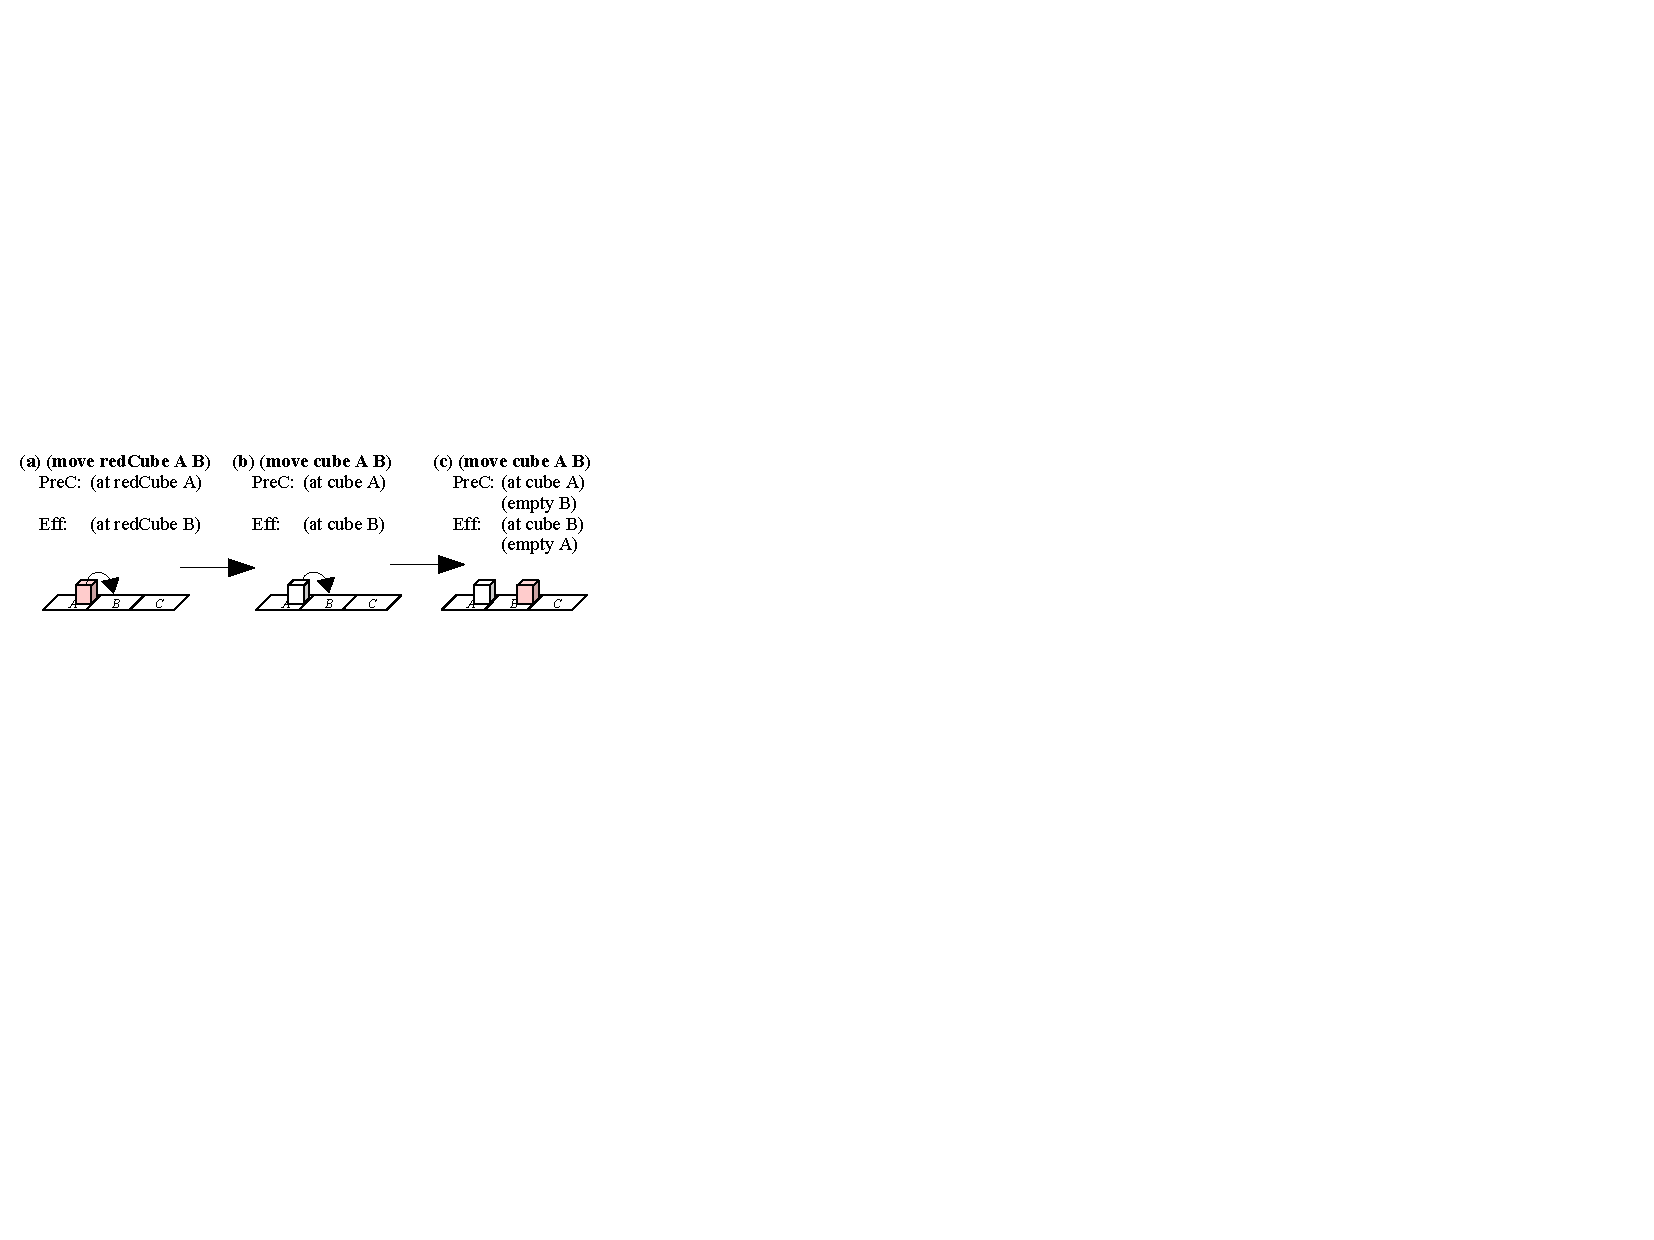
\includegraphics[width=0.8\linewidth]{figures/scenarios-exp2}
	\caption{Continuous refinement of the move action model: (a) initial action model learned by demonstration, (b) action model for all cubes of any colour, (c) action model with an additional condition, if the target position is occupied and cubes can not be stacked.}
	\label{fig:scenarios-exp2}
\end{figure} 

The experiment consisted of the following phases:
\begin{itemize}
  %\item{Introduction: After a short introduction to the Baxter robot \cite{Baxter}, users were told that they needed to use a planning language (STRIPS) to explain Baxter the state of the world and the semantic meaning of the actions.}
  \item{\textbf{Training:} Users were shown how to manipulate Baxter's arm, and given time to familiarise themselves with the kinesthetic manipulation. 
  	For this experiment we only used the robot's suction gripper to manipulate objects.}
  \item{\textbf{Experimental test:} Users were instructed to teach Baxter a move action of a red cube. 
  	Then, they were presented the action model, with preconditions and effects, that Baxter learned from the demonstration (\fig{fig:scenarios-exp2}a). 
  	In the following, users were faced with two different scenarios to refine the conditions of the action model. 
  	Starting with the initial action model for a red cube, users modified the conditions, so that it was applicable to all cubes of any colour (\fig{fig:scenarios-exp2}b), and when the target position was occupied (\fig{fig:scenarios-exp2}c). 
  	At each step, users observed how Baxter executed the learned action in the new scenario. 
  	When Baxter failed to execute the action, users had to refine the conditions of the action model.}
  \item{\textbf{Planning:} Users were presented a new scenario, where Baxter was instructed to achieve a goal using the learned action model. 
  	The new goal was to switch the positions of two cubes on the table (\fig{fig:planning-permutation}). 
  	Users first asked if they believed Baxter was able to solve this task and then shown how the taught action was reused with an automated planner.
  	Finally, Baxter executed the action sequence to complete the task.}
  \item{\textbf{Questionnaire:} Users were given a questionnaire containing 18 questions related to their experience (\eg `I did not encounter any difficulties during the experiment') and their perceived understanding of the presented concepts (\eg `I can explain how Baxter represented the preconditions of a new action'), and the usability of the framework (\eg `No programming experience is required to teach Baxter a new task').
  Participants had to give a rating on a scale ranging from `Strongly agree', `Somewhat agree', `Somewhat disagree', and `Strongly disagree'.
  The complete questionnaire can be found in Appendix \ref{app:exp2}.}
   \item{ \textbf{Debriefing:} Throughout the experiment, users were asked about their expectations on Baxter's behaviour before applying the learned action model to a new scenario. 
   	Users were asked open-ended questions (\eg ``What will Baxter do when applying the learned action model?"), so that their responses were unbiased. 
   	When they encountered failure scenarios (\eg when Baxter stacked two cubes), they were asked to reason about Baxter's behaviour and proposed modifications to the taught action model.} 
\end{itemize}

\subsection{Results}
During the experiments we observed how users learned and used the presented programming process and planning concepts.
When asked for improvements of the initial action model (\fig{fig:scenarios-exp2}a) no users pointed out missing conditions before being faced with the new scenario (\fig{fig:scenarios-exp2}c).
Even users who were `experts' and who have heard of automated planning before, did not propose a complete action model from the start. 
However, when faced with the relevant failure scenarios all users detected the missing conditions easily.
In the final phase, 8 (or 73\%) users with no experience in automated planning did not expect Baxter to solve the permutation problem, and agreed unanimously that it acted in an intelligent manner, when it did. 

Figure \ref{fig:eEvaluation} shows the user responses to the questionnaire.
All (11) users were satisfied with the PbD process and Baxter's abilities to learn and reproduce the demonstrated move action and no users encountered difficulties during the experiment. 
%All users understood the learned action model and managed to adopt the notions of preconditions and effects easily. 
At the end of the experiment, all users believed that they had taught Baxter a new task. 
The majority of users were confident that they could explain how Baxter learned and represented the new action model.
9 (or 82\%) understood the notion of preconditions and agreed that no programming experience was required to teach Baxter using the proposed framework.


\begin{figure}[h]
	\centering
	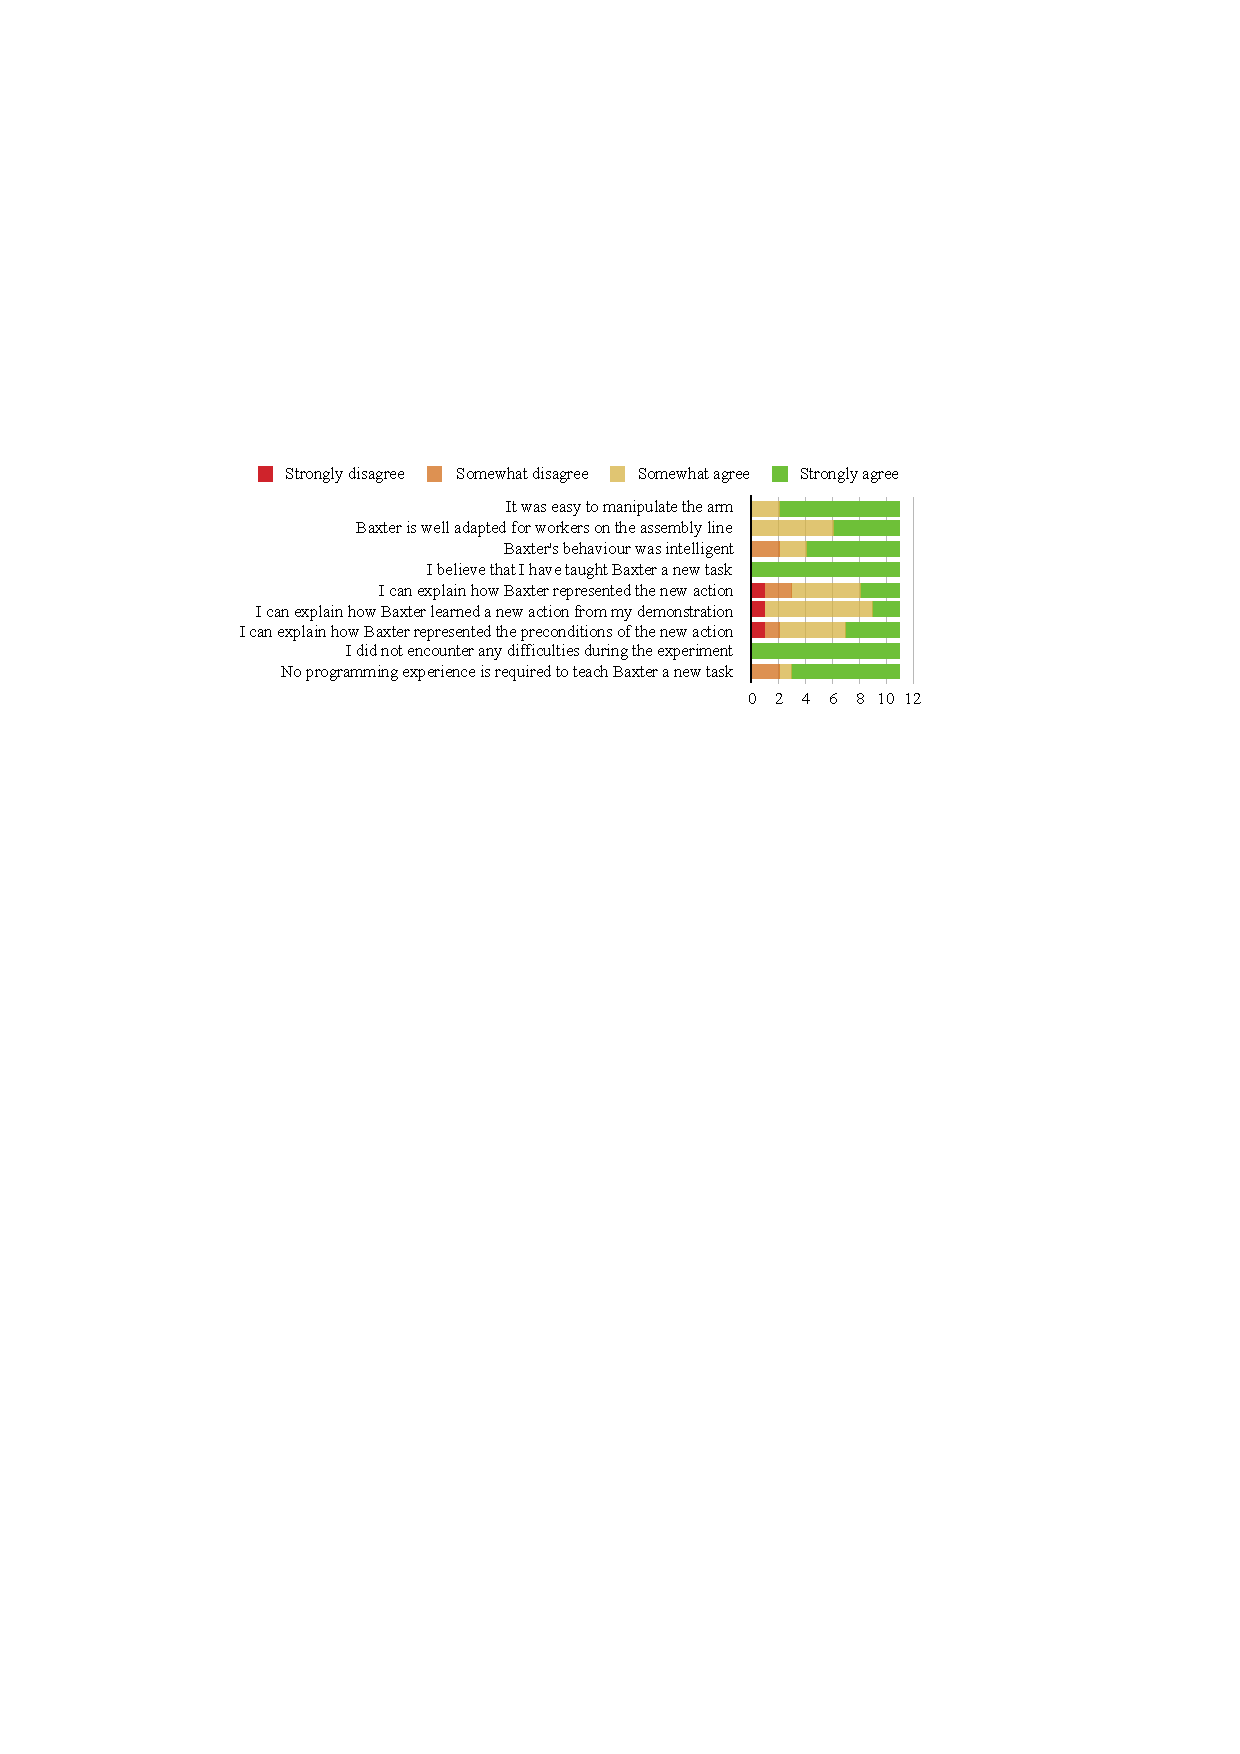
\includegraphics[width=\linewidth]{figures/eEvaluation}
	\caption{Summary of questionnaire responses: Extract of 18 questions on the user's perceived usability and understanding of the programming process after the experiment.}
	\label{fig:eEvaluation}
\end{figure}


\subsection{Discussion and Limitations}
In both experiments, we did not observe a significant difference in the performance between users with different programming experience. The majority of users had issues formulating the logical representations of object properties used in action models. In the first experiments, users had difficulties formulating a single condition (e.g. \texttt{(stackable ball cube)}), but stated equivalent conditions (\textit{`only place the ball, if it is stackable on the cube'}).
Similarly, in the second experiment, users formulated the missing precondition (\textit{`position B is empty'}) with other equivalent conditions (\textit{`Do not place the object on position B, if it is occupied'}). This means, that users should be provided with a predefined set of conditions that can be added to the action model.

Some users made wide assumptions about the robot's capabilities. In the second experiments, when both arrival and departure positions were occupied (Fig. \ref{fig:scenarios-exp2}c), less half of the users (5) expected Baxter to consider the occupied position, even though the condition was not mentioned in its action model.
This is a common problem in PbD solutions as there is a difference in the perception of the robot's intelligence perceived by its teacher (\cite{suay2012practical}) and can be addressed by reproducing the learned task in a new context and verifying the robot's knowledge base, as we did throughout the experiment.

With these two qualitative experiments, we showed that the automated planning language could easily be adopted by users without any programming background. Moreover, the action model representation, in terms of preconditions and effects, seems to be intuitive for non-expert users. 
However, these initial experiments only provide us with an idea of how the users might perceive the proposed framework. We intentionally limited the set of concepts that are necessary to use the framework to the bare minimum. Further experiments should test scalability and address more complicated actions involving separate control groups (experts vs non-experts) in less structured scenarios. 